% TinyTeX here lacks grfext; figures are PDF, so skip the EPS-conversion helper that needs it.
\expandafter\def\csname ver@epstopdf-base.sty\endcsname{2020/01/01}
\documentclass[11pt]{article}
\usepackage[margin=1in]{geometry}
\usepackage{booktabs,graphicx,amsmath,url,natbib}
\usepackage{lmodern}\usepackage[T1]{fontenc}

\title{Think Only When Unsure: One-Pass Confidence Routing Matches\\Reasoning at Half the Tokens on Decision Tasks}
\author{Dheeraj Gadde\\\small Independent researcher \quad \texttt{dhegadde@gmail.com}}
\date{DRAFT, \today}

\begin{document}
\maketitle

\begin{abstract}
We show that a model answering in one pass when it is confident, and reasoning only when it is not, matches
the accuracy of always reasoning at about half the tokens on decision tasks the model never trained on.
Deciding when to reason matters because reasoning-first generation multiplies inference cost, while many
decisions do not need it.
We train a typed decision head (a small scorer over a fixed option set, one forward pass, no generated text)
on Gemma~4 E4B with LoRA and evaluate it, the instruction-tuned model answering directly, and the same model
with its native thinking mode on 10 held-out tasks (1,900 items), with pre-registered predictions.
Routing the least confident questions (about 30\%) to the thinking model gives 80.7 $\pm$ 1.1\% (3 seeds, threshold
chosen on separate data) against 80.8\% for thinking on every question, at 259 versus 521 tokens per question;
the trained head is a modestly better router than the chat model's own answer confidence (about +1 point at
12\% fewer tokens).
Model size mattered more than reasoning: Gemma~4 31B answering in one token (85.7\%) beat E4B thinking (80.8\%).
\end{abstract}

\section{Introduction}
Reasoning before answering (chain-of-thought) improves accuracy on many tasks \citep{wei2023chainofthoughtpromptingelicitsreasoning},
but a meta-analysis found its gains concentrated on math and symbolic problems
\citep{sprague2025cotcotchainofthoughthelps}, and it costs hundreds of generated tokens per question.
For \emph{decisions} (pick one of $K$ options) a product category has emerged around one-pass typed decision
heads, such as TypeSafe AI's Jev, a ``System One Model'' that returns typed decisions with calibrated
probabilities instead of text \citep{jev}. Its makers recommend acting on high-confidence decisions and escalating
the rest; we measure how well that pattern works with open models. This raises a
practical question that neither literature answers directly: on decision tasks, when is one pass enough, and
can a model tell?

We study this with open Gemma~4 models \citep{gemma4} on 10 decision tasks held out from training, comparing
at matched items a trained one-pass head, the instruction-tuned model answering with one letter, and the same
model thinking first, then combining them in a confidence-based cascade in the spirit of FrugalGPT
\citep{chen2023frugalgptuselargelanguage}. All predictions were written down before each run; we report the
ones that failed.

\paragraph{Contributions.}
\begin{itemize}\setlength\itemsep{0pt}
\item A cascade that escalates only low-confidence questions to a thinking model matches always-thinking
  accuracy at $\sim$50\% of the tokens, with the threshold chosen on held-in data (3 seeds).
\item A trained decision head ties a one-letter chat answer in accuracy at similar cost but is better calibrated,
  which makes it a modestly better router than the chat model's own confidence.
\item On these tasks thinking helped more than the prior literature suggested (+3.4 points for E4B), but scale
  helped more: a 31B model answering in one token beat a 4B-class model thinking.
\end{itemize}

\section{Setup}
\paragraph{Tasks.} The head is trained on six decision tasks (BoolQ, SST-2, MNLI, CommonsenseQA, Yelp polarity,
and a synthetic text-coherence task; 2,000 items each) and evaluated on 10 others it never sees: IMDB
\citep{maas-etal-2011-learning}, RTE, MRPC and STS-B (GLUE, \citealp{wang2019gluemultitaskbenchmarkanalysis}),
HellaSwag \citep{zellers2019hellaswagmachinereallyfinish}, ARC-Easy \citep{clark2018thinksolvedquestionanswering},
OpenBookQA \citep{mihaylov2018suitarmorconductelectricity}, WiC \citep{pilehvar2019wicwordincontextdatasetevaluating},
Winogrande \citep{sakaguchi2019winograndeadversarialwinogradschema} and COPA (SuperGLUE,
\citealp{wang2020supergluestickierbenchmarkgeneralpurpose}). STS-B is cast as picking one of six similarity levels.
Generation arms use a fixed random subsample of 200 items per task (COPA: 100), 1,900 in total; averages weight
tasks equally.

\paragraph{Decision head.} Each option is appended to the shared text (``\emph{state} Question: \emph{q} Answer:
\emph{option}'') and the backbone's final hidden state is normalized (LayerNorm without affine parameters) and
scored by a two-layer MLP; a softmax over the $K$ scores gives option probabilities. The backbone is Gemma~4 E4B
with LoRA \citep{hu2021loralowrankadaptationlarge} (rank 16, attention and MLP projections), trained jointly with
the head for 1,500 steps (4 items per step, learning rate $5\times10^{-5}$, warmup-stable-decay schedule). At
$10^{-4}$ training diverged in one run without any numerical overflow (dev accuracy 77\%$\to$29\%); $5\times10^{-5}$
trained cleanly in all three seeds.

\paragraph{Generation arms.} Gemma~4 E4B-it and 31B-it see the text, the question and lettered options, and are
asked for the letter only. \emph{Direct}: thinking off. \emph{Thinking}: the model's native thinking mode, up to
1,024 thinking tokens, after which the answer is forced (1.9\% of E4B items, 9\% of 31B items). In both arms we
read the answer distribution at the answer position, restricted to the option letters, so every arm yields
probabilities. Decoding is greedy.

\paragraph{Tokens.} We count tokens read plus written per question. For the head we count the shared text once
plus each option (93 on average); our first implementation re-reads the shared text per option (205).

\paragraph{Cascade.} The head answers when its top probability is at least $t$, otherwise the thinking model
answers. $t$ is chosen per head seed on 400 in-distribution dev items (the training tasks), maximizing cascade
accuracy, and applied unchanged to the held-out tasks.

\section{Results}

\begin{figure}[t]
\centering
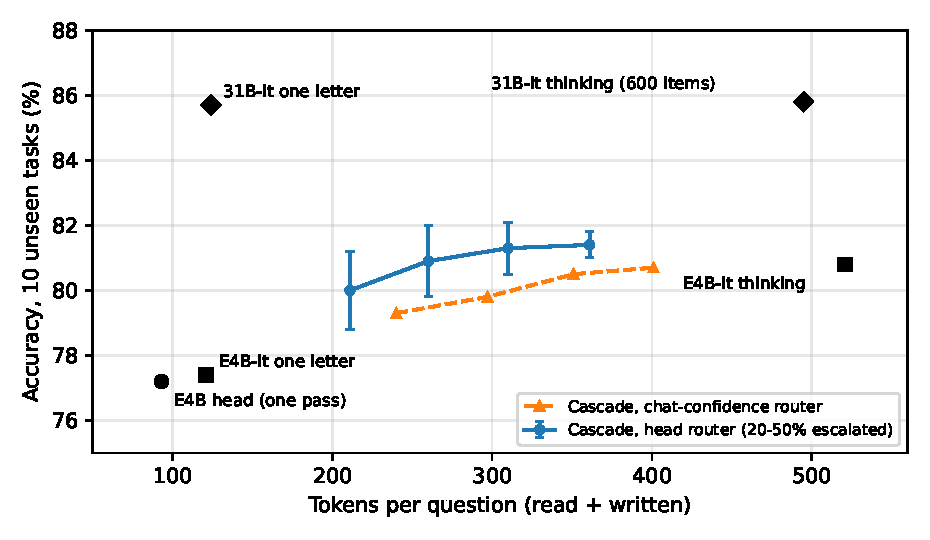
\includegraphics[width=0.82\linewidth]{fig_tokens_accuracy.pdf}
\caption{Accuracy against tokens per question on 10 unseen decision tasks (1,900 items; 31B thinking on a
600-item subset). Cascades escalate the least confident 20--50\% of questions to E4B thinking; error bars are
$\pm$1 s.d.\ over 3 head seeds. A 31B token costs roughly 7$\times$ an E4B token.}
\label{fig:main}
\end{figure}

\paragraph{One pass vs.\ thinking (same model size).} The trained head and the instruction-tuned model's
one-letter answer tie (77.2\% vs 77.4\%; Table~\ref{tab:tasks}); the head is better calibrated (Brier score
0.344 vs 0.385). Thinking adds 3.4 points (80.8\%) at 4.3$\times$ the tokens. The gains are uneven: pronoun
resolution (Winogrande +13), science questions (OpenBookQA +9.5), entailment (RTE +7.5) and word sense (WiC +6),
while story completion (HellaSwag) loses 5. We had predicted a gain below 3 points from
\citet{sprague2025cotcotchainofthoughthelps}; the prediction was narrowly wrong.

\begin{table}[t]
\centering\small
\begin{tabular}{lcccc}
\toprule
Task & E4B head & E4B-it direct & E4B-it thinking & 31B-it direct \\
\midrule
IMDB & 97.5 & 90.5 & 93.0 & 93.5 \\
RTE & 83.5 & 83.0 & 90.5 & 92.0 \\
HellaSwag & 85.0 & 77.5 & 72.5 & 91.0 \\
ARC-Easy & 93.0 & 97.0 & 96.0 & 96.5 \\
OpenBookQA & 72.5 & 84.5 & 94.0 & 97.5 \\
MRPC & 71.0 & 65.5 & 64.0 & 70.5 \\
WiC & 61.0 & 67.0 & 73.0 & 74.5 \\
Winogrande & 68.5 & 66.0 & 79.0 & 88.0 \\
COPA & 97.0 & 95.0 & 98.0 & 98.0 \\
STS-B (6 levels) & 43.0 & 48.0 & 48.0 & 55.5 \\
\midrule
Average & 77.2 & 77.4 & 80.8 & 85.7 \\
Tokens / question & 93 & 121 & 521 & 124 \\
\bottomrule
\end{tabular}
\caption{Accuracy (\%) per held-out task, 200 items each (COPA 100), one run per arm (head: seed 1). With 200
items the standard error per task is about 3 points.}
\label{tab:tasks}
\end{table}

\paragraph{Cascade.} With the dev-chosen threshold, the cascade reaches 82.0, 79.8 and 80.3\% for the three head
seeds (mean 80.7 $\pm$ 1.1\%), escalating 26--32\% of questions, at 259 tokens per question against 521 for
thinking alone (80.8\%). We had predicted the cascade would beat thinking alone for every seed; it matched it.

\paragraph{Is a trained head needed?} Routing by the instruction-tuned model's own probability for its one-letter
answer, at matched escalation rates (no threshold tuning), gives 79.3 / 79.8 / 80.5\% at 20 / 30 / 40\% escalation,
against 80.0 / 80.9 / 81.3\% (s.d.\ about 1) for the head, which also uses about 12\% fewer tokens
(Figure~\ref{fig:main}). The head is a modest improvement, not a requirement.

\paragraph{Scale vs.\ reasoning.} Gemma~4 31B-it answering with one letter reaches 85.7\% (Brier 0.277), above E4B
thinking at a quarter of the tokens, and close to the commercial Jev API on the full test sets of the same tasks (86.8\%). On a 600-item
subset, 31B thinking adds 2.8 points (85.8\% vs 83.0\%). Routing from the E4B head to 31B thinking with the same
thresholds costs about 5 points (80.8 $\pm$ 1.9\% vs 85.8\%): a router much weaker than its fallback keeps answers
the fallback would have fixed. The 31B model routes itself far better: answering with one letter and thinking
only on its least confident 10\% of questions gives 85.0\% at 207 tokens per question against 85.8\% at 495 for
thinking on everything (600 items, matched escalation, no threshold tuning). The strongest model's own one-pass
confidence was the best router we found; a separate small head paid off only when the fallback was its own size.

\paragraph{Reading shared text once.} Encoding the shared text once and reusing its key-value cache for every
option gives the same predictions (99.2\% identical, accuracy 76.8\% vs 76.7\% on all 4,285 held-out items) with
2.2$\times$ fewer tokens. Done one question at a time it ran 5.4$\times$ slower; batched across questions (prefixes
left-padded, cache repeated per option, explicit position ids) it ran 1.5$\times$ faster than the per-option
version on the same GPU (69 s vs 101 s for all 4,285 items, RTX 5090) with the same predictions (99.1\% identical,
76.9\% vs 76.8\%).

\section{Related work}
Cascades that try a cheap model first and escalate on low reliability are established
\citep{chen2023frugalgptuselargelanguage}, as is adapting how much a reasoning model thinks to its confidence
\citep{wang2026conformalthinkingriskcontrol}. Chain-of-thought's benefits outside symbolic tasks are
limited in prompted evaluations \citep{sprague2025cotcotchainofthoughthelps}. Multitask instruction training
transfers to unseen tasks \citep{sanh2022multitaskpromptedtrainingenables,wei2022finetunedlanguagemodelszeroshot},
which our head relies on; distilling rationales into small models is an alternative way to bring reasoning into
one pass \citep{hsieh2023distillingstepbystepoutperforminglarger}. TypeSafe AI recommends the same act-or-escalate use of Jev's confidence \citep{jev} but we found no published
measurement of it (as of September 2026). Our contribution is a matched measurement on
held-out decision tasks, with a trained one-pass decision head as the first stage.

\section{Limitations}
One model family (Gemma~4) and 10 tasks. Each generation arm is a single greedy run; claims other than the
cascade result (3 head seeds) and the E4B-vs-E2B comparison are single-run and should be read as likely rather
than established. 31B thinking covers 600 items. Dev-set thresholds come from the training tasks, not the
held-out ones. Token counts ignore the different cost per token of different model sizes, except where noted,
and shared-prefix timing was measured on one GPU type.

\section*{Reproducibility}
Code, run scripts, per-item outputs and the pre-registered plans are available at \url{https://github.com/dhegadde/think-only-when-unsure}. Total compute
for the experiments in this paper was about \$10 of rented GPU time.

\bibliographystyle{plainnat}
\bibliography{refs}

\appendix
\section{Pre-registered predictions}
\begin{tabular}{p{7.2cm}p{2.3cm}p{4.2cm}}
\toprule
Prediction (written before the run) & Outcome & Observed \\
\midrule
E4B head beats E2B head on held-out tasks by 3--8 points (revised to $-2$ to $+4$) & exceeded & +9.8 to +10.9 (3 seeds) \\
Thinking beats direct by less than 3 points (E4B) & narrowly wrong & +3.4 \\
Trained head beats the same model answering directly & wrong (tie) & 77.2 vs 77.4 \\
Cascade within 2 points of the best arm, $<$40\% escalated & supported & $-$0.1, 30\% escalated \\
Cascade beats thinking alone for all 3 seeds (dev threshold) & wrong & 2 of 3 below \\
Shared-prefix predictions agree $\geq$99.5\% & narrowly wrong & 99.1--99.2\% \\
\bottomrule
\end{tabular}

\end{document}
